%% abtex2-modelo-trabalho-academico.tex, v-1.7.1 laurocesar
%% Copyright 2012-2013 by abnTeX2 group at http://abntex2.googlecode.com/
%%
%% This work may be distributed and/or modified under the
%% conditions of the LaTeX Project Public License, either version 1.3
%% of this license or (at your option) any later version.
%% The latest version of this license is in
%%   http://www.latex-project.org/lppl.txt
%% and version 1.3 or later is part of all distributions of LaTeX
%% version 2005/12/01 or later.
%%
%% This work has the LPPL maintenance status `maintained'.
%%
%% The Current Maintainer of this work is the abnTeX2 team, led
%% by Lauro C\'{e}sar Araujo. Further information are available on
%% http://abntex2.googlecode.com/
%%
%% This work consists of the files abntex2-modelo-trabalho-academico.tex,
%% abntex2-modelo-include-comandos and abntex2-modelo-references.bib
%%

% ------------------------------------------------------------------------
% ------------------------------------------------------------------------
% abnTeX2: Modelo de Trabalho Academico (tese de doutorado, dissertacao de
% mestrado e trabalhos monograficos em geral) em conformidade com
% ABNT NBR 14724:2011: Informacao e documentacao - Trabalhos academicos -
% Apresentacao
% ------------------------------------------------------------------------
% ------------------------------------------------------------------------

%ARQUIVO DE PREAMBULO DA TESE - PACOTES E CONFIGURA\c{C}\~{O}ES

\documentclass[
	% -- op\c{c}\~{o}es da classe memoir --
	12pt,				% tamanho da fonte
	%openright,			% cap\'{\i}tulos come\c{c}am em p\'{a}g \'{\i}mpar (insere p\'{a}gina vazia caso preciso)
	oneside,			% para impress\~{a}o em verso e anverso. Oposto a oneside
	a4paper,		% tamanho do papel.
	% -- op\c{c}\~{o}es da classe abntex2 --
	chapter=TITLE,		% t\'{\i}tulos de cap\'{\i}tulos convertidos em letras mai\'{u}sculas
	%section=TITLE,		% t\'{\i}tulos de se\c{c}\~{o}es convertidos em letras mai\'{u}sculas
	%subsection=TITLE,	% t\'{\i}tulos de subse\c{c}\~{o}es convertidos em letras mai\'{u}sculas
	%subsubsection=TITLE,% t\'{\i}tulos de subsubse\c{c}\~{o}es convertidos em letras mai\'{u}sculas
	% -- op\c{c}\~{o}es do pacote babel --
%	english,			% idioma adicional para hifeniza\c{c}\~{a}o
	%french,			% idioma adicional para hifeniza\c{c}\~{a}o
	%spanish,			% idioma adicional para hifeniza\c{c}\~{a}o
	brazil,				% o \'{u}ltimo idioma \'{e} o principal do documento
	english,
	sumario=tradicional,
	]{abntex2}


% ---
% PACOTES
% ---

% ---
% Pacotes fundamentais
% ---

\usepackage{chngcntr}
\counterwithin{figure}{chapter}
\counterwithin{table}{chapter}
\usepackage{cmap}				% Mapear caracteres especiais no PDF
\usepackage{lmodern}			% Usa a fonte Latin Modern			
\usepackage[T1]{fontenc}		% Selecao de codigos de fonte.
\usepackage[utf8]{inputenc}		% Codificacao do documento (convers\~{a}o autom\'{a}tica dos acentos)
\usepackage{mathptmx}			% Times New Roman font
\usepackage{lastpage}			% Usado pela Ficha catalogr\'{a}fica
\usepackage{indentfirst}		% Indenta o primeiro par\'{a}grafo de cada se\c{c}\~{a}o.
\usepackage{color}				% Controle das cores
\usepackage[pdftex]{graphicx}	% Inclus\~{a}o de gr\'{a}ficos
\usepackage{epstopdf}           % Pacote que converte as figuras em eps para pdf
\usepackage{lipsum}             % Pacote que gera texto dummy
\usepackage{blindtext}          % Pacote que gera texto dummy
% ---
		
% ---
% Pacotes adicionais, usados apenas no \^{a}mbito do Modelo Can\^{o}nico do abnteX2
% ---
\usepackage{nomencl}
\usepackage{amsmath,amssymb,amsfonts,amsthm}
\usepackage{bbm}
\usepackage[chapter]{algorithm}
\usepackage{multirow}
\usepackage{rotating}
\usepackage{pdfpages}
\usepackage{gensymb}
% ---

\usepackage{algorithm}



% ---
% Pacotes de cita\c{c}\~{o}es
% ---
\usepackage[alf,abnt-etal-cite=2,abnt-etal-list=3,abnt-etal-text=emph,abnt-emphasize=bf]{abntex2cite}
\newcommand{\citet}{\citeonline}
%Cita\c{c}\~{o}es padr\~{a}o ABNT
%\citeoption{abnt-full-initials=no,abnt-url-package=url}
% ---
% Pacote de customiza\c{c}\~{a}o - Unicamp
% ---
\usepackage{unicamp}

% Pacotes necesitados por Aldo Díaz
\usepackage{enumitem}
\usepackage{array}
\usepackage{longtable}
\usepackage{mathtools}
\usepackage{tikz}
\usepackage[noend]{algpseudocode}
\usepackage{xr}

% ---
% CONFIGURA\c{C}\~{O}ES DE PACOTES
% ---

\renewcommand{\ABNTEXchapterfont}{\fontfamily{ptm}\fontseries{b}\selectfont}
\renewcommand{\ABNTEXchapterfontsize}{\large}
\renewcommand{\ABNTEXsectionfont}{\fontfamily{ptm}\fontseries{b}\selectfont}
\renewcommand{\ABNTEXsectionfontsize}{\normalsize}
\renewcommand{\ABNTEXsubsectionfont}{\fontfamily{ptm}\selectfont}
\renewcommand{\ABNTEXsubsectionfontsize}{\normalsize}

%\makeatletter
%\newcommand\thefontsize[1]{{#1 The current font size is: \f@size pt\par}}
%\makeatother


\externaldocument[1-]{cap1_intro}
\externaldocument[2-]{cap2_teoria}
\externaldocument[3-]{cap3_metodo}
\externaldocument[5-]{cap6_validation}
\externaldocument[6-]{cap4_results}
\externaldocument[7-]{cap5_conclu}

\newcolumntype{L}[1]{>{\raggedright\let\newline\\\arraybackslash\hspace{0pt}}m{#1}}
\newcolumntype{C}[1]{>{\centering\let\newline\\\arraybackslash\hspace{0pt}}m{#1}}
\newcolumntype{R}[1]{>{\raggedleft\let\newline\\\arraybackslash\hspace{0pt}}m{#1}}

\DeclarePairedDelimiter\ceil{\lceil}{\rceil}
\DeclarePairedDelimiter\floor{\lfloor}{\rfloor}
\newcommand{\Conv}{\mathop{\scalebox{1.5}{\raisebox{-0.2ex}{$\ast$}}}}
\usetikzlibrary{shapes.geometric, arrows}
%\floatname{algorithm}{Algoritmo}

\tikzstyle{startstop} = [rectangle, rounded corners, minimum width=3cm, minimum height=1cm,text centered, draw=black, fill=gray!20]
\tikzstyle{io} = [trapezium, trapezium left angle=70, trapezium right angle=110, minimum width=3cm, minimum height=1cm, text centered, text width=5cm, draw=black]
\tikzstyle{process} = [rectangle, minimum width=3cm, minimum height=1cm, text centered, text width=3cm, draw=black]
\tikzstyle{decision} = [diamond, minimum width=3cm, minimum height=1cm, text centered, draw=black]
\tikzstyle{arrow} = [thick,->,>=stealth]

% ---
\ifpdf % used graphic file format for pdflatex
  \graphicspath{{./eps/}}
  \DeclareGraphicsExtensions{.png,.jpg,.pdf}
\else  % used graphic file format for latex
  \DeclareGraphicsExtensions{.eps}
\fi

%customiza\c{c}\~{a}o do negrito em ambientes matem\'{a}ticos
\newcommand{\mb}[1]{\mathbf{#1}}
%customiza\c{c}\~{a}o de teoremas
\newtheorem{mydef}{Defini\c{c}\~{a}o}[chapter]
\newtheorem{lemm}{Lema}[chapter]
\newtheorem{theorem}{Teorema}[chapter]


% ---
% Configura\c{c}\~{o}es de apar\^{e}ncia do PDF final

% alterando o aspecto da cor azul
\definecolor{blue}{RGB}{41,5,195}

% informa\c{c}\~{o}es do PDF
\makeatletter
\hypersetup{
     	%pagebackref=true,
		pdftitle={\@title},
		pdfauthor={\@author},
    	pdfsubject={\imprimirpreambulo},
	    pdfcreator={LaTeX with abnTeX2},
		pdfkeywords={abnt}{latex}{abntex}{abntex2}{trabalho acad\^{e}mico},
		hidelinks,					% desabilita as bordas dos links
		colorlinks=false,       	% false: boxed links; true: colored links
    	linkcolor=blue,          	% color of internal links
    	citecolor=blue,        		% color of links to bibliography
    	filecolor=magenta,      	% color of file links
		urlcolor=blue,
%		linkbordercolor={1 1 1},	% set to white
		bookmarksdepth=4
}
\makeatother
% ---

% ---
% Espa\c{c}amentos entre linhas e par\'{a}grafos
% ---

% O tamanho do par\'{a}grafo \'{e} dado por:
\setlength{\parindent}{2.0cm}

% Controle do espa\c{c}amento entre um par\'{a}grafo e outro:
\setlength{\parskip}{0.2cm}  % tente tamb\'{e}m \onelineskip

% ---
% Informacoes de dados para CAPA e FOLHA DE ROSTO
% ---
\titulo{Sistema de Decolagem e Pouso de Precisão com Quadrotor Autônomo Usando Detecção de Tags Aruco e Redes Neurais Convolucionais}
\autor{Alan Ferreira Pinheiro Tavares}
\local{Campinas}
\data{2018}
\orientador{Prof. Dr. Paulo Roberto Gardel Kurka}
%\coorientador[Co-orientador]{Prof. Dr. Co-orientador}
\instituicao{%
    UNIVERSIDADE ESTADUAL DE CAMPINAS
    \par
    Faculdade de Engenharia Mecânica	
    }
%\tipotrabalho{Tese (Doutorado)}
%% O preambulo deve conter o tipo do trabalho, o objetivo, o nome da institui\c{c}\~{a}o e a \'{a}rea de concentra\c{c}\~{a}o
%\preambulo{Tese apresentada \`{a} Faculdade de Engenharia El\'{e}trica e de Computa\c{c}\~{a}o da Universidade Estadual de Campinas como parte dos requisitos exigidos para a obten\c{c}\~{a}o do t\'{\i}tulo de Doutor em Engenharia El\'{e}trica, na \'{A}rea de Engenharia de Computa\c{c}\~{a}o.}
\tipotrabalho{Disserta\c{c}\~{a}o (Mestrado)}
\preambulo{Dissertation presented to the School of Mechanical Engineering of the University of Campinas in partial fulfillment of the requirements for the Master's degree, in the field of Solid Mechanics and Mechanical Design.\\ \hfill \\Disserta\c{c}\~{a}o apresentada \`{a} Faculdade de Engenharia Mec{\^a}nica da Universidade Estadual de Campinas como parte dos requisitos exigidos para a obten\c{c}\~{a}o do t\'{\i}tulo de Mestre em Engenharia Mec{\^a}nica, na \'{A}rea de Mecânica dos Sólidos e Projeto Mecânico.}

% --- 


% ---- compila o \'{\i}ndice  ----
\makeindex
%\makenomenclature
% ---
%\usepackage{titlesec, blindtext, color}
%\newcommand{\hsp}{\hspace{20pt}}
%\titleformat{\chapter}[hang]{\Huge\bfseries\uppercase}{\thechapter{. }}{0pt}{\Huge\bfseries}
% ---- In\'{\i}cio do documento ----
\begin{document}

% Retira espa\c{c}o extra obsoleto entre as frases.
\frenchspacing

\makepagestyle{abntheadings}
\makeevenhead{abntheadings}{\ABNTEXfontereduzida\thepage}{}{\ABNTEXfontereduzida\textit\leftmark}
\makeoddhead{abntheadings}{}{}{\ABNTEXfontereduzida\thepage}

% ---- ELEMENTOS PR\'{E}-TEXTUAIS ----
\pretextual

%\pagenumbering{roman}

% --- Capa ---
\imprimircapa
% ---

% --- Folha de rosto (o * indica que haver\'{a} a ficha catalogr\'{a}fica) ---
\setcounter{page}{2}

\imprimirfolhaderosto*
% ---

% --- Inserir a ficha catalogr\'{a}fica ---
 \begin{fichacatalografica}
    \centering
    %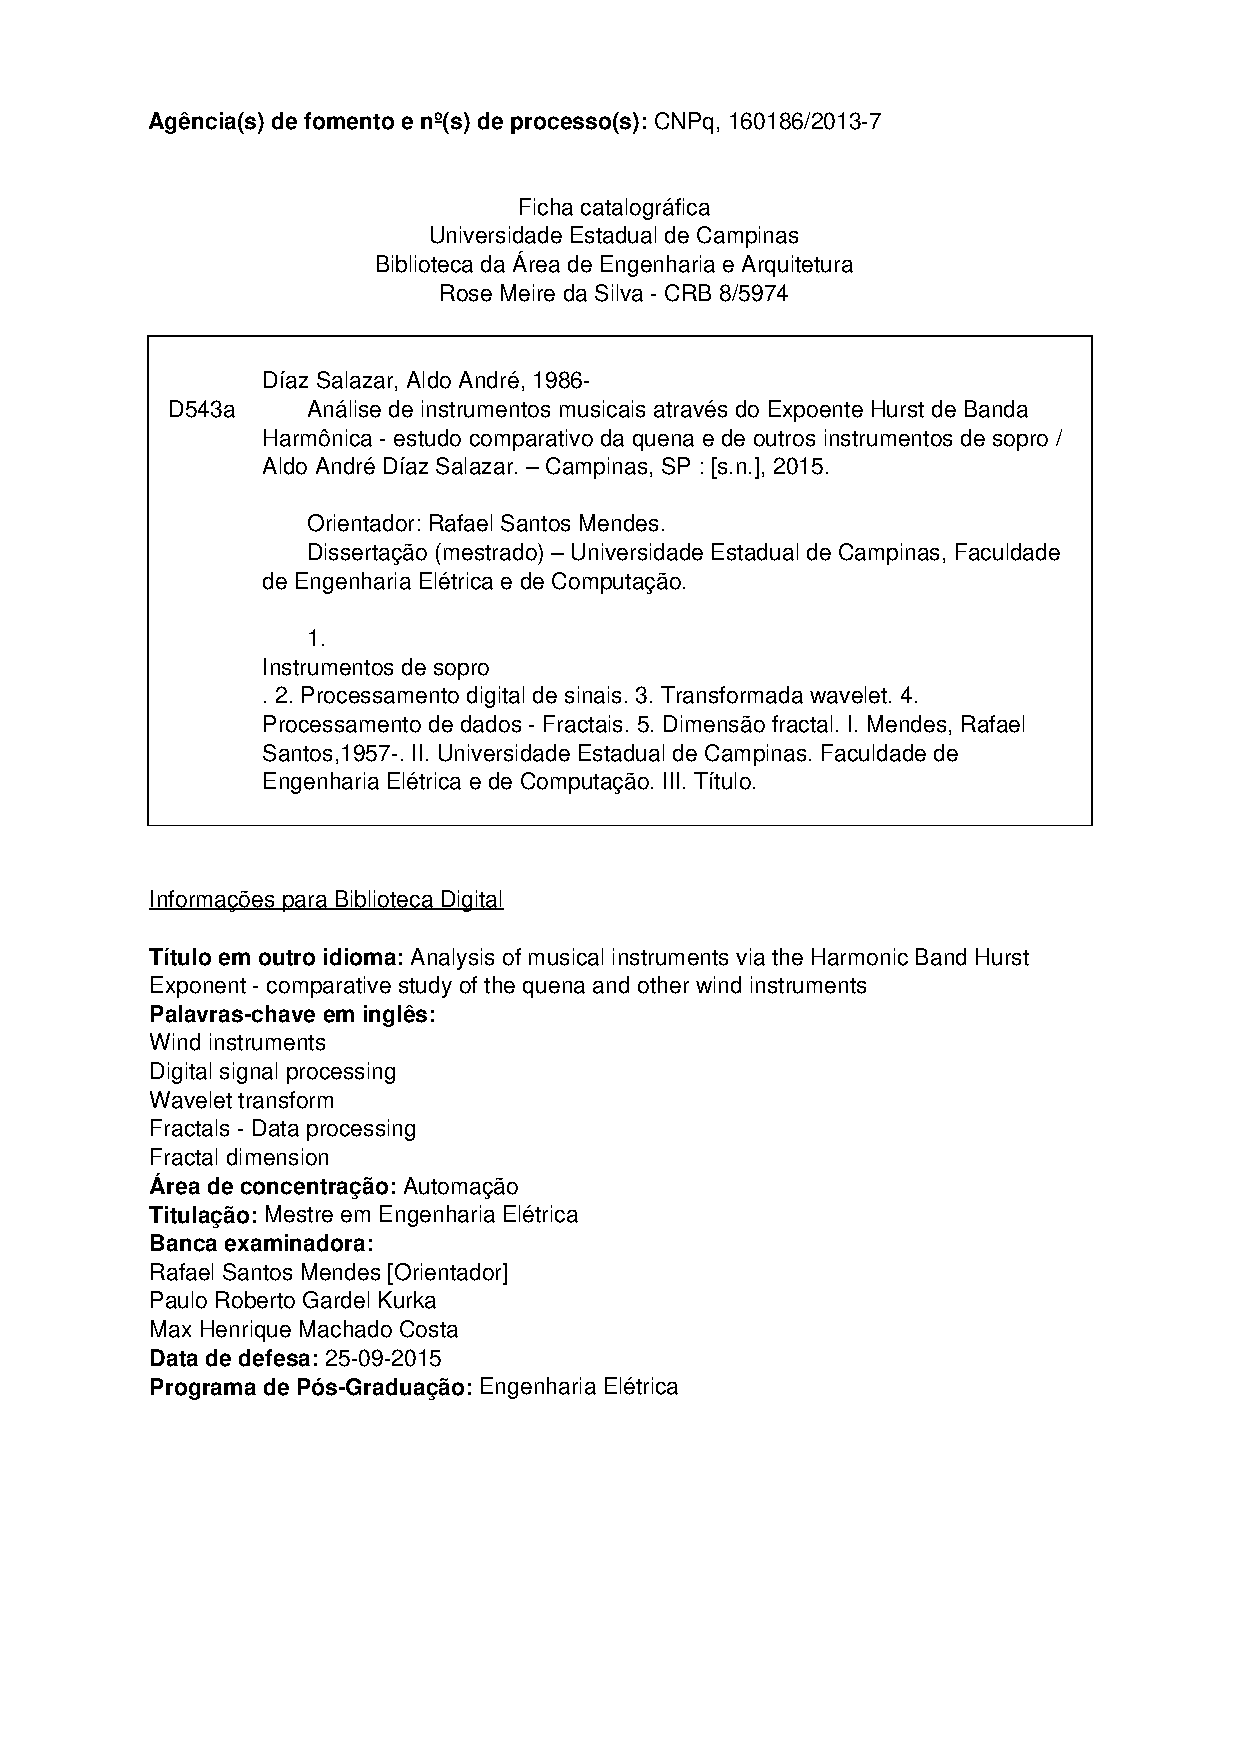
\includepdf{ficha-catalografica.pdf}
 \end{fichacatalografica}

\newpage
\begin{center}\large\textbf{UNIVERSIDADE ESTADUAL DE CAMPINAS \\
		FACULDADE DE ENGENHARIA MECÂNICA \\
		COMISSÃO DE PÓS-GRADUAÇÃO EM ENGENHARIA MECÂNICA \\
		DEPARTAMENTO DE SISTEMAS INTEGRADOS
		}\end{center}	
\vspace{0cm}	
\begin{center}\textbf{DISSERTAÇÃO DE MESTRADO ACADÊMICO}\end{center}
\vspace*{0cm}
\begin{center}
	\Huge\textbf{\imprimirtitulo}
\end{center}
\begin{flushleft}
Autor: \imprimirautor 
\\
Orientador: \imprimirorientador \\
\hfil \\
A Banca Examinadora composta pelos membros abaixo aprovou esta Dissertação:
\\ \hfil \\
\textbf{Prof. Dr. Marco Lucio Bittencourt \\
FEM/UNICAMP \\
\hfil \\
Prof. Dr. Gregory Bregion Daniel  \\
FEM/UNICAMP \\
\hfil \\
Prof. Dr. Francisco José Profito  \\
PME/EPUSP}

\hfil \\
A Ata da defesa com as respectivas assinaturas dos membros encontra-se no processo de vida acadêmica do aluno.
\end{flushleft}
\vspace{0.2cm} 
\begin{flushright}
	Campinas, 04 de agosto de 2017.
\end{flushright}
\newpage

% --- --- ---

%\cleardoublepage

% --- Dedicat\'{o}ria ---
\begin{dedicatoria}
    \vspace*{\fill}
    \centering
    \noindent
    \textit{À minha família,\\
    	    que mesmo longe, esteve sempre comigo. }
    \vspace*{\fill}
\end{dedicatoria}
% ---

% --- Agradecimentos ---
\begin{otherlanguage*}{brazil}
\begin{agradecimentos}
Gostaria de agradecer, primeiramente, aos meus pais, Ana e Valter, que me apoiaram em todos os momentos e que conhecem os caminhos que me levaram até aqui. Foi a estrada que vocês trilharam que me trouxe tão longe e onde ela começa é o lugar que chamarei sempre de lar. Obrigado também à minha irmã Jocasta e à minha prima Thais, por fazerem parte dos ótimos momentos que uso de recordação e inspiração. 

Agradeço imensamente ao professor Marco Lúcio Bittencourt, pela chance de fazer parte desse projeto. O aprendizado proporcionado por esse mestrado estará comigo sempre e se hoje dou mais um passo em direção à pesquisa, é porque ele me deu a oportunidade e me inspirou a continuar buscando o conhecimento sempre.

Deixo aqui também um agradecimento especial ao professor Francisco José Profito. Sem a sua ajuda, eu não teria chegado tão longe nessa pesquisa. Muito obrigado pelas conversas e pelas dúvidas respondidas.  

Muito obrigado a todos do lab, por tornarem a experiência do mestrado muito mais tranquila e divertida. Alfredo, obrigado pelo template em LATEX, mas também por dividir os problemas e alegrias do mestrado comigo. Guilherme, muito obrigado por toda a ajuda no início da minha pesquisa, em especial pelo suporte na utilização dos softwares comerciais de simulação. Darla e Mari, muito obrigado pelo convívio e pela dose de humor e loucura quase diária. Eduardo, obrigado pela ajuda a cada novo documento que precisava ser entregue e pela companhia nas reuniões de projeto. Agradeço imensamente a todos e espero o melhor para vocês.

Agradeço eternamente aos meus conterrâneos e amigos, Alessandro, Breno e Lívia, que passaram pelas mesmas dificuldades e saudades que passei para virem até aqui e que estiveram comigo durante toda essa jornada. Vocês foram essenciais para tornar essa jornada mais fácil e saibam que, aonde quer que estejamos, poderão sempre contar comigo.     

Meu muito obrigado àquela que esteve comigo durante todos os momentos. Cintia, meu amor, obrigado por fazer parte dessa história e dividir comigo os melhores momentos. Você foi e vai ser sempre minha referência do melhor que posso ser. Seu apoio foi vital para minha sanidade durante esse mestrado. Obrigado por estar comigo na alegria e na tristeza, na saúde e na doença, na pobreza e na menos pobreza, por todos os dias.

Por fim, meus agradecimentos ao professor Waldyr Luiz Ribeiro Gallo, pela gerência do projeto temático, e à Fundação de Amparo à Pesquisa do Estado de São Paulo (FAPESP) pela concessão do auxílio à pesquisa e bolsa de mestrado.  

	
	
\end{agradecimentos}
\end{otherlanguage*}
% ---

% --- Ep\'{\i}grafe  ---
%\begin{epigrafe}
%    \vspace*{\fill}
%    \begin{flushright}
%        \textit{``To be born ignorant is nobody's fault, but to remain is everybody's responsibility.''\\
%        (Abraham Laboriel, Músico profissional)}
%    \end{flushright}
%\end{epigrafe}
% ---

% --- RESUMOS (em portugu\^{e}s e ingl\^{e}s ---
\begin{otherlanguage*}{english}
	\begin{center}{\ABNTEXchapterfont\ABNTEXchapterfontsize RESUMO}\end{center}

Em 2009, 56 milhões de litro de combustível foram gastos com o atrito em motores de combustão, sendo os mancais responsáveis por cerca de um quarto dessa perda. Essa pesquisa tem o objetivo de modelar numericamente os mancais de um virabrequim com alívio de peso, estudando os efeitos que a texturização superficial desses mancais pode ter no seu desempenho e focando em reduzir o atrito deste componente. Uma revisão bibliográfica foi realizada, tratando da texturização superficial, dos regimes de lubrificação e aspectos de rugosidade, contato de superfícies e temperatura. Um programa de computador foi desenvolvido para estudar o comportamento de um mancal carregado dinamicamente, levando em conta efeitos de rugosidade, contato de asperezas, efeitos térmicos e texturização superficial. Simulações foram realizados no mancal de um virabrequim com alívio de peso, aplicando diferentes designs de textura à sua superfície. Os resultados mostraram que é possível reduzir o coeficiente de atrito hidrodinâmico médio e máximo destes componentes, mas alguns designs de texturas tendem a aumentar a pressão no fluido lubrificante, especialmente se forem levados em conta os efeitos térmicos.  

\noindent\textbf{Palavras-Chave}: Texturização Superficial; Equação de Reynolds; Regime de Lubrificação Mista; Mancal de Deslizamento; 

\end{otherlanguage*}

\newpage
\begin{resumo}
	Text abstract...

\vspace{\onelineskip}

\noindent\textbf{Keywords}: Surface Texture; Reynolds Equation; Mixed Lubrication;Crankshaft Journal Bearings; Roughness Effects.
%sound analysis; Harmonic Band Hurst Exponent; wind instruments; quena.

\end{resumo}



\newpage
% ---

\renewcommand{\listfigurename}{List of Figures}
\renewcommand{\listtablename}{List of Tables}
\renewcommand{\contentsname}{Contents}
\renewcommand{\figurename}{Fig.}
\renewcommand\bibname{References}
\renewcommand\tablename{Table}

% --- inserir lista de ilustra\c{c}\~{o}es ---
\pdfbookmark[0]{\listfigurename}{lof}
\listoffigures*
\cleardoublepage
%% ---
%
%% --- inserir lista de tabelas ---
\pdfbookmark[0]{\listtablename}{lot}
\listoftables*
\cleardoublepage
% ---


%\begin{siglas}
%	\item[Fig.] Area of the $i^{th}$ component
%	\item[456] Isto é um número
%	\item[123] Isto é outro número
%	\item[lauro cesar] este é o meu nome
%\end{siglas}


% inserir lista de símbolos
% ---
\begin{simbolos}
	\item[$ a, b, c $] Constants for the dynamic viscosity thermal models
	\item[$ x, y, z $] Cartesian axis
	\item[$ u_x, u_y, u_z $] Local velocity components
	\item[$ r_x, r_y, r_z $] Elliptical dimple radius
	\item[$ x_c, y_c, z_c $] Elliptical dimple origin center
	\item[$ h $] Fluid film thickness
	\item[$ h_o $] Radial clearance
	\item[$ h' $] Mean surface separation
	\item[$ h_T $] Film thickness between two rough surfaces
	\item[$ t $] Time
	\item[$ e $] Eccentricity
	\item[$ k $] Successive over relaxation iteration step		
	\item[$ q_x, q_z $] Lubricant film flow	
	\item[$ n_x, n_z $] Number of dimples
	\item[$ P $] Hydrodynamic pressure
	\item[$ P_{cav} $] Cavitation pressure
	\item[$ P_{amb} $] Ambient pressure	
	\item[$ R $] Bearing radius
	\item[$ R_j $] Journal radius
	\item[$ U, W $] Rotational speeds on the x and y axes.
	\item[$ T $] Temperature in Kelvin
	\item[$ T_{\circ C} $] Temperature in Celsius
	\item[$ C_p $] Lubricant specific heat
	\item[$ Q $] Axial fluid film flux
	\item[$ E $] Combined elastic modulus
	\item[$ N $] Number of asperities
	\item[$ N_x, Nz $] Number of integration points
	\item[$ L_x $] Bearing thickness
	\item[$ L_z $] Bearing length
	\item[$ L_{tx}, L_{tz} $] Length of dimple cell	
	\item[$ W_x, W_y $] Length of dimple cell	
	\item[$ F_x, F_y $] Length of dimple cell			
	\item[$ Z_s $] Mean asperity height of combined rough surfaces	
	\item[$ \mu $] Dynamic viscosity
	\item[$ \rho $] Lubricant density
	\item[$ \rho_c $] Lubricant density on cavitation pressure
	\item[$ \tau $] Shear stress
	\item[$ \varepsilon $] Eccentricity ratio
	\item[$ \beta $] Bulk modulus
	\item[$ \beta_s $] Mean asperity radius of combined rough surfaces
	\item[$ \sigma_r $] Standard deviation of combine roughness amplitude 
	\item[$ \sigma_s $] Standard deviation of asperity heights 
	\item[$ \delta_r $] Combined roughness amplitude
	\item[$ \eta_s $] Asperity density
	\item[$ \vartheta $] Dissipated power
	\item[$ \zeta $] Friction torque
	\item[$ \omega_p $] Over relaxation parameter for the pressure
	\item[$ \omega_p $] Over relaxation parameter for the film fraction
	\item[$ \xi_{p} $] Pressure tolerance
	\item[$ \xi_{\theta} $] Film fraction tolerance
	\item[$ \xi_{x} $] Tolerance for the support load on the $x$ axis
	\item[$ \xi_{y} $] Tolerance for the support load on the $y$ axis
	\item[$ \xi_{T} $] Temperature tolerance
	\item[$ \Lambda$] Ratio between fluid film thickness and surface roughness	
	\item[$ \phi_{p_{(x,z)}} $] Patir and Cheng pressure flow factors
	\item[$ \phi_{s_{(x)}} $] Patir and Cheng shear flow factors
	\item[$ \phi_{fp_{(x,z)}}$] Patir and Cheng friction pressure flow factors
	\item[$ \phi_{fs_{x}}$] Patir and Cheng friction shear flow factors
	\item[$ \phi_{f_{(x,z)}}$] Friction contact factor	
			
\end{simbolos}
% ---

% --- inserir lista de Algorítimos ---
%\pdfbookmark[0]{\listalgorithmname}{las}
%\listofalgorithms
%\cleardoublepage
% ---

% --- inserir o sumario ---

\pdfbookmark[0]{\contentsname}{toc}
\addtocontents{toc}{\protect\setcounter{tocdepth}{1}}
\tableofcontents*


\cleardoublepage
% ---

% --- inserir lista de Acronimos e Abrevia\c{c}\~{o}es ---
%\renewcommand{\nomname}{Lista de Acr\^{o}nimos e Abrevia\c{c}\~{o}es}
%\pdfbookmark[0]{\nomname}{las}
%\printnomenclature
%\cleardoublepage
% ---

\pagenumbering{arabic}

% ---- ELEMENTOS TEXTUAIS ----
\textual
\setcounter{page}{4}  %Colocar contador acordo com a numeracao do texto
% ---- Introdu\c{c}\~{a}o ----

%\part{Introdução}
\chapter{Introdução}

\section{Motivação}

O uso de Veículos Autônomos Aéreos Não Tripulados (VAANTs), também conhecidos como \textit{drones} ou quadrotores autônomos, vêm ganhando notoriedade nas últimas décadas devido à sua alta versatilidade, manobrabilidade, avanço tecnológico computacional, seguido também de aplicações inovadoras em quase todos os setores, sejam elas com propósito militar, de pesquisa, comércio, vigilância ou de lazer. Justifica-se também este interesse por conta do crescente número de fabricantes, redução de preços, melhoria da qualidade dos componentes e sensores envolvidos, demandando assim técnicas mais robustas para garantir a segurança das aeronaves \cite{Santos2014}.

Segundo definições de \citet{Duan2010}, VAANT é um tipo de sistema muito complexo que integra diferentes componentes de hardware, como o Sistema de Posicionamento Global (GPS), Unidade de Gerenciamento Inercial (IMU), controlador e diferentes componentes de software, como processamento de imagem e planejamento de trajetória. \citet{Costa2012} destaca a importância da IMU no sistema de localização dos VAANTs que integra bússola, barômetro, sonares e sensor GPS. Tanto o IMU quanto a bússola indicam a atitude; Barômetro e sonar podem ser usados para leitura de altitude, e o GPS para obter dados de posicionamento e também altitude. 

\subsection{Problematização da Descolagem e Pouso}

Contudo, estes sensores de navegação podem apresentar erros da ordem de metros e de forma acumulativa, principalmente quando se diz a respeito de pousos ou decolagens utilizando GPS próximos a prédios, redes elétricas ou montanhas que bloqueiam ou anulam completamente o sinal de GPS. Este fato deprecia a qualidade, confiabilidade e custo da missão, visto que se faz necessário a aquisição de sensores com altíssima precisão e com blindagem eletrostática específica, resultando em custo elevado. Logo, a visão computacional é uma excelente solução de baixo custo e alto retorno de informações espaciais para o controle de VAANTs.
 
Tal solução é apresentada através das câmeras de sensor exteroceptivo ou monocular, que além de atribuir precisão em navegação possui a vantagem de ser um sensor passivo, de baixa sensibilidade a ruídos e independente do sinal de GPS, permitindo voo em ambientes onde esse sinal não possui boa qualidade \cite{GUO2014}. Pode-se citar algorítimos de código aberto como de \citet{Forster2014} e \citet{Raul2016}, que trazem robustas soluções de navegação por visual monocular através de uma abordagem semi-direta que elimina a necessidade de extração de recursos caros e técnicas de correspondência robustas para estimativa de posição e orientação.

%===================================================================================================

\subsection{Aplicação de Drones em Serviçoes de encomendas \textit{(delivery)}}

Uma das aplicações dos estudos desta tecnologia está presente no setor de encomendas \textit{(delivery)}, onde são utilizados pelo serviço de entregas em algumas regiões como nos Estados Unidos, Austrália e Suíça. Um dos exemplos é o serviço \textit{Prime Air} da companhia \textit{Amazon}, que promete atender a encomendas de até 5 \textit{libras} em meia hora, com veículos cobertos de redundâncias "\textit{sense and avoid}" para garantir a segurança durante o tráfego em rotas especiais. Na Suíça estão sendo testados \textit{drones} para entregas de encomendas pesando até um quilograma por distâncias que se estendem a dez quilômetros, segundo notícias de Agosto de 2016 \cite{Vidal2016}.

Segundo notícias de Maio de 2018. O Brasil já realizou a primeira simulação de \textit{delivery}, que ocorreu em São Paulo com autorização do Departamento de Controle do Espaço Aéreo (DECEA). Com o objetivo de entregar medicamentos, a ação utilizou um hexacóptero e um programa desenvolvidos pela marca nacional \textit{SMX Systems}. Apesar de ser considerada a primeira simulação oficial, esta não foi a primeira vez em que uma entrega é feita com \textit{drone} no país, já que em 2014 houve um \textit{delivery} de pizza no município de Santo André (SP) \cite{Techtudo2018}.


\subsection{Problematização Linhas de Transmissão}

Segundo \citet{Gilberto2016} Uma das principais limitações dos VAANTs em praticamente todos os tipos de aplicações é a carga útil limitada que eles podem carregar. Esta situação limita a quantidade de baterias transportadas durante uma missão que, consequentemente, restringe o tempo de voo. Devido a essa limitação, os veículos voadores precisam retornar a uma estação de recarga após um curto período de operação. Neste contexto, a aterrissagem autônoma torna-se essencial para economizar energia em missões do tipo \textit{perch-and-stare} em que a manutenção do voo não é necessariamente necessária. Além disso, ao realizar tarefas em que seja necessário um voo longo contínuo ou viagens de longa distância, o retorno a uma estação base não é prático. Nesses cenários, seria mais conveniente implantar uma estação base móvel capaz de transportar energia suficiente para vários ciclos de recarga. Os VAANTs, então, teriam que realizar pouso periódico autônomo em estações de ancoragem baseadas em terra ou voadoras para recarregar e se tornar operacional novamente.

\subsection{Sugestão da Solução}

Com base nos argumentos descritos acima, verifica-se a motivação da tesa no âmbito de desenvolver e simular um sistema para VAANT do tipo quadrotor capaz de aterrissar de forma autônoma um alvo pré-definido e estático. A tese visa realizar o controle do VAANT usando apenas sensoriamento por visão e computação embarcada, sem depender de qualquer infraestrutura externa. A simulação é feita via V-REP usando linguagem \textit{Python} e captura de imagem monocular. O algorítimo inicialmente detecta o local de decolagem/pouso via marcador fiducial \textit{tag} \textit{ArUco}, em seguida retorna a posição do quadrotor em relação ao marcador, contornando erros inerentes a sensores de posicionamento, como IMU e GPS. O diferencial da proposta baseia-se em obter um algorítimo que utilize a Rede Neural Convolucional (CNN) de forma a complementar a detecção da \textit{tag} \textit{ArUco} clássica da maneira mais eficaz. Deseja-se criar dados de treinamento híbridos através de dados sintéticos e reais de forma a superar a limitações de casos específicos como detecção imprecisa a longa distância, oclusão parcial ou uso de câmeras com alta distorção. 

Verifica-se a utilização de \textit{ArUco} pelo fato de ser uma biblioteca de código aberto para detecção de marcadores fiduciais. Segundo \citet{Aruco2014}, a biblioteca permite estimar a pose de uma câmera a partir de um ou vários marcadores que são analisados em paralelo, onde, cria-se uma imagem canônica no nível da pirâmide que alcança o melhor equilíbrio entre qualidade e tamanho, sendo atualmente uma das estratégias mais investigas para uso como marcador de pouso e rastreamento com VAANTs, além de dispor de criação de marcadores personalizados. 

%Contudo, tem-se ainda o desafio de identificação a longo alcance, visto que o marcador fiducial tem um limite de tamanho por distancia de identificação segura. Ou seja, para alturas elevadas acima de 30 metros se faz necessário o uso de uma segunda abordagem, um algoritmo de odometria visual monocular que mesmo sem a identificação do marcador, guie o \textit{drone} próximo a altura de identificação segura. 

%===================================================================================================

%Logo o trabalho traz a proposta de se utilizar a biblioteca ArUco  em conjunto com o algorítimo de \citet{Forster2014}, uma técnica já consolidada e precisa que segundo o autor a mais rápida dos métodos atuais de última geração. Tem-se como vantagem, a abordagem semi-direta que elimina a necessidade de extração de recursos caros e técnicas de correspondência robustas para estimativa de movimento. O algorítimo opera diretamente nas intensidades de pixel, o que resulta em precisão de subpixel em altas taxas de quadros. Chamado pelo autor como abordagem de \textit{Odometria Visual Semi-Direta} (SVO), já foi testado em veículos micro-aéreos e lançado como \textit{software} de código aberto.

%Em relação ao desafio de custo elevado versos desempenho computacional, conta-se com a estratégia de embarcar o \textit{software} desenvolvido em um \textit{hardware} de dispositivo \textit{smartphones} via plataforma \textit{Android} com o objetivo obter desempenho computacional bom ou similar a computadores convencionais quando utilizados para o mesmo objetivo. As vantagens de se embarcar uma interface \textit{Android} é facilidade de comunicação e uso dos periféricos já embarcados no dispositivo, além dos ganhos em custo benefício entre processamento e consumo de energia.

%Por fim, serão realizados testes experimentais que verifiquem o desempenho do sistema desenvolvido frente a 2 (duas) abordagens utilizadas para pouso de precisão: 1.PX4Flow via técnica Optical Flow; 2.IR-LOCK via câmera PIXY. Estima-se o uso do sistema em uma aplicação real em missões de entregas (\textit{deliveries}) de medicamento na cidade do Porto-Portugal vinculada a empresa \textit{Connec Robotics}. As mesmas técnicas utilizadas para o pouso bodem ser replicadas para a decolagem que também apresenta grandes problemáticas quando guiada somente por GPS. 

%\subsection{Objetivo}

%O presente trabalho tem como objetivo principal desenvolver e simular um sistema de decolagem e pouso de precisão autônoma para um VAANT do tipo quadrotor. A tese visa realizar o controle do sistema utilizando somente técnicas de visão computacional simuladas via V-REP usando um quadrotor com câmera monocular. O algorítimo inicialmente detecta o local de decolagem/pouso via marcador fiducial \textit{tag} ArUco, em seguida retorna a posição do quadrotor em relação ao marcador, contornando erros inerentes a sensores de posicionamento, como IMU e GPS. O diferencial da proposta baseia-se em obter um algorítimo que utilize a Rede Neural Convolucional (CNN) de forma a complementar a detecção da \textit{tag} ArUco clássica da maneira mais eficaz. Deseja-se criar dados de treinamento híbridos através de dados sintéticos e reais de forma a superar a limitações de casos específicos como detecção imprecisa a longa distância, oclusão parcial ou uso de câmeras com alta distorção.

\vspace{\fill}

%\begin{itemize}
    
    %A metodologia adotada demanda as seguintes etapas:
    
  %\item Realizar levantamento bibliográfico sobre os principais conceitos e desafios de pesquisa referentes a pouso e decolagem de precisão autônoma utilizando veículos quadrotores;
  
  %\item Embarcar bibliotecas de OpenCV, ArUco e \textit{Tensorflow}  vinculados a linguagem de programação C/C++ ou \textit{Python} em uma única IDE;
  
  %\item Estruturar um dicionário de marcadores fiduciais que apresente bons desempenhos nos quesitos de identificação precisa do marcador e confiabilidade de posição;
  
  %\item Desenvolver inicialmente um algorítimo que tenha como saída a posição do marcador de pouso em relação ao quadrotor, baseada somente na técnica de detecção via \textit{tag} ArUco;
  
  %\item Utilizar o Simulador V-REP para integrar a comunicação de controle do quadrotor com o algorítimo desenvolvido;
  
   %\item Realizar a aquisição de dados sintéticos de treinamento de rede neural através de ensaios simulados de decolagem e pouso com quadrotores via V-REP;
  
  %\item Realizar a aquisição de dados reais de treinamento de rede neural através de ensaios reais de decolagem e pouso com quadrotores via gravações de \textit{datasets};
   
   %\item  Realizar treinamento dos dados obtidos para identificar o marcador desejado utilizando técnica de Rede Neural Convolucional (CNN);
   
   %\item Implementar e simular no V-REP o algorítimo desenvolvido (CNN) de forma a complementar a detecção da \textit{tag} ArUco clássica da maneira mais eficaz.
   
   %\item Coletar dados estatísticos dos ensaios simulados via V-REP e analisar o desempenho do sistema autônomo projetado;
   
    %\item Determinar os melhores parâmetros visando eficiência na identificação de marcadores a longa distância, onclusões parciais e distorção de câmera;
    
%\end{itemize}

%===================================================================================================

\section{Estado da Arte}

%\subsection{Visão Geral: Veículos Autônomos Aéreos Não Tripulados VAANTS}

	%\subsubsection{Conceitos e Fundamentos}

	%\subsubsection{Desafios de Controle e Navegação em Pouso/Decolagem}

	%\subsubsection{Aplicações Comerciais}

%\subsection{Trabalhos Relacionado: Descolagem e Pouso Autônomo}

	%\textbf{Revisão Literária das Principais Técnicas de Decolagem e Pouso}

	%\textbf{Revisão Literária do Uso de Marcadores Fiduciais como \textit{Landmarks}}

	%\textbf{Revisão Literária das Técnicas de Redes Neurais Usadas para Aperfeiçoar a Detecção de \textit{Tags} ArUco}
	
	Neste tópico, será abordado uma revisão literária sobre as principais técnicas utilizadas para decolagem e pouso de precisão para VAANT do tipo quadrotor, bem como, os principais trabalhos que utilizam técnicas para detecção de marcadores visuais como solução do problema de localização. Priorizou-se técnicas que utilizaram somente visão computacional a fim de criar um estado da arte mais próximo do proposta pela tese, a qual visa contornar erros inerentes a sensores de posicionamento como IMU e GPS ou sensores ativos como lasers e sonares. 
	
	O entendimento dessas técnicas é exposta de forma resumida através da Tabela~\ref{qd:estado-da-arte}, onde, destaca-se a principal abordagem e contribuição científica de cada referência. Em seguida, realiza-se uma análise comparativa destes trabalhos em relação ao trabalho proposto e os principais desafios superados por cada técnica, sendo o principal objetivo deste tópico. 
	
    \begin{table}[H]
    \centering
	\caption{Resumo das principais abordagens e contribuições científicas relacionadas à decolagem e pouso de VANTs usando somente visão computacional.}
	%\vspace{0.5cm}
	\begin{tabular}{ccc}
		   
	\hline
	\multirow{2}{*}{\textbf{Abordagem}} & \multirow{2}{*}{\textbf{Contribuição}} & \multirow{2}{*}{\textbf{Referências}} \\
	\\ \hline
	\multirow{3}{*}{Odometria Monocular}  & \multirow{3}{*}{Sistema de Pouso Autônomo} &  \\
	\multirow{3}{*}{Estimação da Plataforma} &  \multirow{3}{*}{em Plataforma Móvel}  & \multirow{2}{*}{\citet{Falanga2017}} \\
	&                                  &                         &                       \\ \hline
	\multirow{3}{*}{Modelo de Controle}  & \multirow{3}{*}{Geração de Trajetória de Pouso} &  \\
	\multirow{3}{*}{Preditivo (MPC)} &  \multirow{3}{*}{e Robustez do Controlador}  & \multirow{2}{*}{\citet{Gilberto2016}} \\
	&                                  &                         &                       \\ \hline
	\multirow{3}{*}{Marcador QR-Code}  & \multirow{3}{*}{Pouso Autônomo Preciso} &  \\
	\multirow{3}{*}{GPS + Navegação Ótica} &  \multirow{3}{*}{em Relação ao GPS Isolado}  & \multirow{2}{*}{\citet{Maiman2017}} \\
	&                                  &                         &                       \\ \hline
	\multirow{3}{*}{Visão Computacional}  & \multirow{3}{*}{Pouso Autônomo} &  \\
	\multirow{3}{*}{Operações Morfológicas} &  \multirow{3}{*}{Somente Técnicas de Visão}  & \multirow{2}{*}{\citet{Vidal2016}} \\
	&                                  &                         &                       \\ \hline
	\multirow{3}{*}{Orientação de Navegação}  & \multirow{3}{*}{Geração de Trajetórias de Pouso} &  \\
	\multirow{3}{*}{Intrínseca de Tau} &  \multirow{3}{*}{ Baseado Espaço-Temporal em 4D}  & \multirow{2}{*}{\citet{Vetrella2017}} \\
	&                                  &                         &                       \\ \hline
	\end{tabular}

	\label{qd:estado-da-arte}
\end{table}

    A literatura sugere que a maioria das implementações de técnicas para decolagem e pouso disponíveis podem ser classificadas em 2 (duas) categorias: A primeira com sistemas que fazem uso de sensores de imagem e a segunda com sistemas cujas capacidades de navegação são baseadas em sensores ativos, como lasers, sonares em casos de ambientes internos e IMU e GPS em casos de ambiente externo.
    
    Destaca-se inicialmente o trabalho de \citet{Falanga2017}, que traz uma abordagem prática, contando com um algorítimo de visão computacional avançado, fusão de multi-sensores para localização do veículo aéreo além de detecção e estimativa de movimento da plataforma móvel usando uma segunda câmera. O algorítimo de detecção visual da plataforma móvel é aplicado em um filtro de \textit{Kalman} atrelado ao modelo cinemático da plataforma, resultando em uma identificação da plataforma móvel com alta frequência.
    
    O principal diferencial entre o trabalho de \citet{Falanga2017} e a tese apresentada é em relação a estratégia de detecção do marcador visual, que não utiliza redes neurais convolucionais. A principal contribuição do trabalho de \citet{Falanga2017} são os resultados práticos do pouso autônomo, que diferente da proposta da presente tesa, visa um pouso em uma plataforma móvel, tendo como maior diferencial a utilização de um rápido algorítimo de odometria monocular de \cite{Forster2014}.
    
    Outro trabalho de relevância é o de \citet{Gilberto2016}, que também tem como objetivo a realização prática de pouso em plataforma móvel, contudo, utilizando micro-veículos aéreos (MAVs). Verifica-se também uma abordagem diferente do proposto pela presente tese, a qual é voltada ao desenvolvimento de um algorítimo de controle através do Modelo de Controle Preditivo (MPC). Esta abordagem considera o problema da robustez de uma forma viável do ponto de vista da implementação do sistema, tendo como principal contribuição científica a geração de uma trajetória ótima, projetada para melhorar o desempenho do controlador e garantir robustez no sistema.
    
    Ainda referente a trabalhos com pouso autônomo, destaca-se o trabalho de \citet{Maiman2017}, que cria uma nova solução precisa e econômica para pouso com \textit{drones}. Diferente do objetivo proposto pela presente tese, o algorítimo desenvolvido por \citet{Maiman2017} chamado de \textit{GOLD} combina GPS com navegação ótica para reconhecer e descer de forma iterativa em direção a um ponto de pouso alvo o qual é identificado via detecção QR-Code. O trabalho traz como contribuição científica um pouso autônomo de baixo custo e mais preciso do que um sistema que utilize somente GPS.
    
    Verifica-se o trabalho de \citet{Vidal2016} relevante para identificar os conceitos essenciais de um sistema de pouso autônomo que utiliza somente técnicas de visão computacional. O trabalho traz uma abordagem de visão computacional pura, utilizando somente técnicas de obtenção de contorno e reconhecimento de formas por operações morfológicas, \textit{thresholding} e outras técnicas matemáticas a fim de se obter processamento rápido e simples. O diferencial entre o trabalho de \citet{Vidal2016} e a tese apresentada é a técnica de detecção visual do marcador que não utiliza marcadores fiducial do tipo \textit{Tag} como \textit{ArUco}, \textit{AprilTag}, \textit{ARToolkit}, \textit{ARTag} ou \textit{QR-Code} e nem detecção avançada por rede neural. Tendo como contribuição científica a validação e implementação de técnicas simples e de rápido processamento em visão computacional, voltada para identificação de contorno e reconhecimento de forma por morfologia para pouso de \textit{drones} autônomos.
    
    No trabalho de \citet{Vetrella2017}, desenvolveu-se um algoritmos flexível de geração de trajetória, sua contribuição científica permitiu altos níveis de autonomia para as fases críticas da missão, como decolagem, cobertura de área e pouso. Diferente da tesa apresentada, o trabalho de \citet{Vetrella2017} apresenta uma abordagem de orientação que usa a teoria de orientação intrínseca da \textit{Tau} aprimorada para criar trajetórias espaço-temporais em 4D para um tempo-para-contato desejado com uma plataforma de aterrissagem rastreada por um sensor visual.
    
    A principal motivação de usar sensores de imagem é seu peso leve e baixo consumo de energia. Para este fim, a literatura sugere várias abordagens que utilizam marcadores visuais para simplificar a problema de localização, como exemplo, têm-se o trabalho de \citet{Pestana2016}, que faz uso de marcadores visuais \textit{ArUco} \citet{Salinas2013}, a abordagem proposta por \citet{Jayatilleke2013} que requer um conhecimento prévio de todas as poses de referência, enquanto que em \citet{Faigl2013}, o VAANT é necessário para manter os marcadores externos sempre visíveis. Nessas abordagens, o uso de marcadores visuais fornece uma localização precisa, com a desvantagem de alterar a área a ser explorada.
    
    Marcadores planares quadrados tornaram-se um método popular para estimar poses em aplicações como robôs autônomos \citet{Robert2009}, \citet{Pichler2017} e \citet{Valencia2005}, veículos não tripulados, \citet{Broggi2000}, \citet{Patterson2014} e \citet{Gonzalez2017}, além de treinadores virtuais \citet{Pflugi2017}, \citet{Chen2016} e \citet{Khattak2014}. Os marcadores permitem estimar a posição de uma câmera monocular com custo mínimo, alta robustez e velocidade. Basta criar marcadores com uma impressora normal, colocá-los no ambiente desejado para cobrir a área de trabalho e registrar sua localização a partir de um conjunto de imagens.
    
    Outras abordagens baseadas em sensores de imagem para realizar a navegação e localização, evitar colisões são os trabalhos de \citet{Zingg2010} e \citet{Lippiello2011}, onde \textit{Pyramidal Lukas-Kanade} é usado para a estimativa do fluxo óptico. As técnicas utilizam informações computadas por algoritmos de fluxo óptico para obter um mapa de profundidade.
    
    Outras abordagens interessantes e mais inovadoras usam o Redes Neurais para classificação e navegação de cenas internas \citet{Kim2015}, utilizando uma \textit{Convolutional Neural Network} (CNN) para aprender uma estratégia de controle baseada em dados capturados de vôos realizados por um piloto especialista humano.
    
    %abordagem que utiliza marcadores fiduciais clássicos ...abordagem que utiliza PX4Flow via técnica Optical Flow e IR-LOCK via câmera PIXY. 
    

%===================================================================================================

\section{Contribuição Científica}
    
    Na presente tese, apresenta-se um sistema validado por simulação via V-REP para VAANT do tipo quadrotor capaz de decolar e pousar de forma autônoma em um alvo estático. O algorítimo é baseado somente em técnicas de visão computacional para detectar a plataforma de pouso através de marcador fiducial e assim retornar a posição do quadrotor em relação ao marcador que foi desenvolvido para ter identificação única. Logo, não há necessidade de nenhum conhecimento prévio sobre a localização da plataforma de pouso. O sistema apresenta baixo custo por eliminar a necessidade de instalação de infraestrutura externa, como um sistema de captura de movimento, além de contornar erros inerentes a sensores de posicionamento, como IMU e GPS. O algorítimo utiliza Rede Neural Convolucional (CNN) de forma a complementar a detecção da \textit{tag} \textit{ArUco} clássica da maneira mais eficaz e supera as limitações da detecção imprecisa a longa distância, oclusão parcial ou uso de câmeras com alta distorção.

	%\subsection{Dicionário de Marcadores para Pouso/Decolagem de Identificação Única}

	%\subsection{Utilização da (CNN) para Complementar a detecção da \textit{tag} ArUco de forma Eficaz}

	%\subsection{Desenvolvimento de um Sistema de Baixo Custo para Decolagem e Pouso Autônomo de Quadrotores sem uso de GPS ou IMU}

\section{Estruturação da Tese}

Os capítulos seguintes descrevem o trabalho da seguinte forma: O capítulo 2 (dois) apresenta o marcador fiducial utilizado como plataforma de pouso, descrevendo seus principais conceitos; O capítulo 3 (três) aborda sobre a técnica de rede neural utilizadas complementarmente na detecção da plataforma de pouso; O capítulo 4 (quatro) descreve o ambiente de simulação, expondo a plataforma usada e as características do veículo aéreo e controlador utilizado; O capítulo 5 (cinco) define as tarefas realizadas e apresenta os resultados e discussões; Por fim, o capítulo 6 (seis) aborda todas as conclusões do trabalho realizado e sugestões de trabalhos futuros.






% ---- Cap\'{\i}tulos ----

%\part{Fundamentos teóricos}

\chapter{Marcadores Fiduciais}

\section{Definição}

\section{Tipos de de Marcadores}

ref = {http://www.scielo.br/scielo.php?script=sci_arttext&pid=S1982-21702014000300626}

\section{\textit{Augmented Reality: Aruco 3}}

\section{Dicionário de Marcadores Proposto}

%\part{Metodologia}

\chapter{Redes Neurais}

\section{Definição}
\textbf{Aprendizagem Supervisionada} \\
1) Tabela de Entradas/Saídas = Aplicações = Técnicas (Tabela Exemplificando)
2) Dados estuturados / Dados Não Estruturados
 
 \textbf{Tipos} \\
 - Standart NN
 - CNN
 - RNN
 - Custom Hybrid
 
 \textbf{Regressão Logística} \\
 Dada uma entrada X(imagem), elabora-se um algorítimo que possa produzir uma previsão que chamaremos de Y(chapeu)=probabilidade que é uma estimatíva de Y.
 
 Tudo se basea em um modelo probabilistico onde Y fica entre 0 e 1
 
 
    
\section{Redes Neurais Convolucionais}

\section{Técnica de Fusão entre Aruco e CNN}


%\part{Resultados}

\chapter{Ambiente de Simulação/Real}

\section{Programa de Simulação Visual}

\section{Plataforma Selecionada para Interface}

\section{Robô Selecionada}

	\subsection{Características do Robô}

	\subsection{Tipo de Controlador}
    
\section{Simulação do Ambiente: Inspeção Autônoma das Redes de Transmissão}

	\subsection{Parâmetros de Simulação}
    
    \subsection{Ambiente de Decolagem e Pouso}
    
    \subsection{Trajetória das Redes de Energia}

\chapter{Resultados de Simulação/Real}

\section{Definição das Tarefas Realizadas (Missões)}

\section{Apresentação dos Resultados}

	\subsection{Marcadores Fiduciais com Redes Neurais Convolucionais}

	\subsection{Algorítimo de Decolagem e Pouso Autônomo}

\section{Discussão dos Resultados}

\section{Crítica dos Resultados}

\chapter{Conclusão}

\section{Observações Finais}

\section{Trabalhos Futuros}

% --- Finaliza a parte no bookmark do PDF, para que se inicie o bookmark na raiz ---
\bookmarksetup{startatroot}%
% ---


% ---- ELEMENTOS P\'{O}S-TEXTUAIS ----
\postextual

% ---- Refer\^{e}ncias bibliogr\'{a}ficas ----

\bibliography{Teste}

% ---- Ap\^{e}ndices ----

% ---
% Inicia os ap\^{e}ndices
% ---
%\begin{apendicesenv}
%
%% Imprime uma p\'{a}gina indicando o in\'{\i}cio dos ap\^{e}ndices
%\partapendices
%
%% ----------------------------------------------------------
%\chapter{Quisque libero justo}
%% ----------------------------------------------------------
%
%\lipsum[50]
%
%% ----------------------------------------------------------
%\chapter{Nullam elementum urna vel imperdiet sodales elit ipsum pharetra ligula
%ac pretium ante justo a nulla curabitur tristique arcu eu metus}
%% ----------------------------------------------------------
%\lipsum[55-57]
%
%\end{apendicesenv}
% ---

% ---- Anexos ----

% ---
% Inicia os anexos - opcional
% ---
%\begin{anexosenv}

% Imprime uma p\'{a}gina indicando o in\'{\i}cio dos anexos
%\partanexos

% ---
%\chapter{Morbi ultrices rutrum lorem.}
% ---
%\lipsum[30]

% ---
%\chapter{Cras non urna sed feugiat cum sociis natoque penatibus et magnis dis
%parturient montes nascetur ridiculus mus}
% ---

%\lipsum[31]

% ---
%\chapter{Fusce facilisis lacinia dui}
% ---

%\lipsum[32]

%\end{anexosenv}

% ---- INDICE REMISSIVO ----

\printindex

\end{document} 
